\chapter{Design}
\section{Language}

The TML provides commands to specify tape operations. In particular, 
\begin{itemize}
    \item we make use of \texttt{move} commands to move the tapehead pointer in some direction; and
    \item we make use of \texttt{changeto} commands to change the tapehead value to some letter in the alphabet.
\end{itemize}
To abstract states in a TM, the TML provides a PL-like alternative, called \emph{modules}. A module simulates a state in TMs. To allow for flow of code to go from one module to another, we make use of \texttt{goto} commands. We can go to the \textit{accept} and \textit{reject} states using the keywords \texttt{accept} and \texttt{reject} respectively.

The following program illustrates a simple program in TML with all the basic operations.
\lstinputlisting[language=TML]{code/simple_program.txt}
The execution of a program starts at the first module, i.e. the module \texttt{first}. We remove the first tape value and move the tape pointer to the right. We then go to module \texttt{second} and continue execution. Note that we allow recursion- line 5 can be replaced with \texttt{goto first}.

To abstract the transition function, the language makes use of \emph{pattern-matching}. To resemble a traditional PL, we make use of \texttt{if} commands. This is shown in the example below.
\lstinputlisting[language=TML]{code/pattern_matching.txt}

Although the language is already equivalent to TMs, TML programs do not abstract TMs enough. In particular, modules are equivalent to TM states at this point. To mitigate this, we add nesting within \texttt{if} statements. That way, modules are more expressible than states. It also allows us to write programs that are more comparable to programs written in other languages. An example of a nested TML program is given below.
\lstinputlisting[language=TML]{code/isDiv2Rec.txt}
In this program, we have nested an \texttt{if} block within an \texttt{if} block in lines 12-15.

\begin{figure}[htb]
    \centering
    \begin{tikzpicture}
        \node[state, accepting] (q0) at (0, 0) {$q_0$};
        \node[state] (q1) at (2.5, -1.3) {$q_1$};
        \node[state, fill=green, opacity=0.6] (A) at (2.5, 1.3) {$A$};
        \node[state, fill=red, opacity=0.6] (R) at (5, -1.3) {$R$};

        \draw[->] (q0) -- node[above, rotate=20] {$0|\#, R$} (A);
        \draw[->] (q0) -- node[below, rotate=-20] {$1, R$} (q1);
        \draw[->] (q1) edge[loop below] node {$0|1, R$} (q1);
        \draw[->] (q1) -- node[below] {$\#, L$} (R);
    \end{tikzpicture}
    \caption{A TM with a self-loop at the state $q_1$.}
    \label{fig:self-loop-TM}
\end{figure}
Although nesting has made the language more like a typical PL, this is not enough. In particular, if we have a self-loop at a non-starting state, then the program cannot be written compactly. To see this, consider the TM at Figure \ref{fig:self-loop-TM}. Currently, the following is the only way to convert this TM into a TML program.
\lstinputlisting[language=TML]{code/forced_complete_program.txt}
What we have is a \emph{complete program}- this is a class of TML programs that are used to \textit{represent} TMs. In particular, 
\begin{itemize}
    \item there is a bijection between TMs and complete TML programs, and
    \item we can easily convert a module to a state, and vice versa.
\end{itemize}
It is not possible to combine the 2 modules- because the block corresponding to $q_1$ would be nested within $q_0$, recursion would convert the self-loop at $q_1$ into a transition from $q_1$ to $q_0$. By only allowing the TM to be written this way, we would not have completely abstracted TM states. We must support nested self-loops.

To allow for self-loops to be nested, we introduce a new construct- a \texttt{while} command. This is similar to an \texttt{if} command, but after the block is executed, we stay at the same block. Note that this does not necessarily mean that the same \textit{case} is run. This is precisely a self-loop. We can now convert the TM to a single module:
\lstinputlisting[language=TML]{code/while_program.txt}
We can also conclude that the TML is not a mere \textit{representation} for TMs- we have found 2 programs that convert to the TM at Figure \ref{fig:self-loop-TM}. So, there is no bijection between TML programs and TMs. We have successfully abstracted TM states and transitions from the language!

The formal syntax of the language is given in the appendix, along with a proof of equivalence between TMs and TML programs in terms of tape execution. The proof of equivalence is composed of several proofs, which involve:
\begin{itemize}
    \item converting a TM into a (complete) TML program;
    \item converting a valid TML program into a complete TML program; and
    \item converting a complete TML program into a TM program.
\end{itemize}

\section{Parser}
The parser takes a program in TML and produces a corresponding TM. It also allows for the execution of a TML program, and a TM, on a tape. It does so in many steps.

\subsection{Lexical Analysis}
The first stage of parsing is lexical analysis, where we produce a stream of tokens from the source code. Since the TML is quite simple, this was decided to be unnecessary- we make use of a stream of \emph{source code}.

\subsection{Syntactic Analysis}

\begin{figure}[htb]
    \centering
    \begin{tikzpicture}[
        level 1/.style={sibling distance=4.5cm}
    ]
        \node[draw, ellipse] {PROGRAM}
        child[
            level 2/.style={sibling distance=1cm}
        ] {
            node[draw, ellipse] {ALPHABET}
            child {
                node[draw] {\texttt{a}}
            }
            child {
                node[draw] {\texttt{b}}
            }
        }
        child[
            level 2/.style={sibling distance=3cm}
        ] {
            node[draw, ellipse] {MODULE}
            child {
                node[draw] {\texttt{first}}
            }
            child {
                node[draw, ellipse] {BASIC-BLOCK}
                child {
                    node[draw, ellipse] {CHANGETO}
                    child {
                        node[draw] {\texttt{blank}}
                    }
                }
                child {
                    node[draw, ellipse] {MOVE}
                    child {
                        node[draw] {\texttt{left}}
                    }
                }
            }
        };
    \end{tikzpicture}
    \caption{An AST for the TML program with a module called \texttt{first}.}
    \label{fig:TML_AST}
\end{figure}

Next, the stream of source code is parsed into an AST. The AST has a node for each command. We illustrate this process with an example. So, assume we have the following source code.
\begin{lstlisting}[language=TML]
alphabet={a, b}
module first {
    changeto blank
    move left
}
\end{lstlisting}
Then, the parsing process results in the construction of the AST given in Figure \ref{fig:TML_AST}. 

The parser is top-down in nature. In particular, when parsing the program above, we try to construct the AST from the root and then fill out the branches and the leaves. Because the language does not have complex parsing rules, we also make use of predictive parsing. In particular, we construct the AST given above as follows:
\begin{enumerate}
    \item We first parse it as a program and construct the root node of the AST;
    \item We detect the alphabet at line 1, so we construct the alphabet branch in the AST; and 
    \item We parse the module \texttt{first} from line 2- we construct the module branch and parse its body.
\end{enumerate}
If successful, this process will result in an AST.

If the parser cannot construct an AST, then the program has some syntax error. In that case, the parser throws an error with a clear and a succinct message.

\subsection{Semantic Analysis}
After the AST has been constructed, we perform semantic analysis. The TML does not have a type system, meaning that we do not need to do type checking. On the other hand, the language makes use of identifiers, e.g. module names. So, we perform scope checking in this stage. This is done by traversing the AST once.

During this phase, we ensure that a \texttt{goto} command refers to a module that is already present in code. By design, we allow the module to be defined anywhere within the document. Moreover, we check that a module is not defined twice, and is not called \texttt{accept} or \texttt{reject}. We also validate that the letter of a \texttt{changeto} command is one of the letters in the \texttt{alphabet} or \texttt{blank}. 

Moreover, there is also a check to ensure that a switch block contains precisely one case for each letter in the alphabet. That is,
\begin{itemize}
    \item there are no duplicate cases present, and 
    \item the cases check all the letters, including \texttt{blank}.
\end{itemize}

\subsection{TM Generation}
Next, the AST is used to generate a TM. This is the final stage of the compilation process. There are many choices to represent a TM, including the formal definition of TMs and the FSM representation. To allow for more flexibility during code execution, the formal definition of TMs was chosen. 

This process is different to the one described in the proof of equivalence- here, we are directly converting a valid TML program into a TM. In essence, we have combined the two steps given in the proof to achieve this.

Initially, we define a TM. During the traversal of the AST, we fill it with relevant states and transitions. This mostly takes place when we are at a block, either inside a module or an \textit{if} command. The process depends on the type of block we have:
\begin{itemize}
    \item if we have a \textit{switch} block, then we define the transition function one by one for each letter, by visiting all the cases within the block;
    \item if we have a \textit{basic} block, then we define the transition function for all the letters in one go.
\end{itemize}
We have commands within the block/case that we can use to define the transition. For instance, if we have the command \texttt{move left}, then the transition direction will be left. If the command is not present, then we add the default transition, as specified in the language specification.

\subsection{TML Execution}

The AST is also used for executing a TML program on a tape. This is the final stage of the interpretation process. Since a TML program is compiled to a TM, this stage could have been avoided- we could make use of executing TM on a tape. However, this was also included since the execution of a TML program was thought to be more efficient. This is because TML program abstracts TM operations. For example, in TMs, each letter in a state should have a different transition, whereas TML supports the same transition for every letter.

The execution of a TML program follows the rules given in the specification. This is included in the appendix. Similarly, the execution of a TM follows the rules given in the background section.

\section{Product}
\subsection{Structure}
The website was planned to have multiple pages, which included:
\begin{itemize}
    \item the \emph{homepage} that allows the user to make use of the parser;
    \item the \emph{documentation pages} that explains TMs and TML programs; along with
    \item the \emph{error pages} to illustrate syntax and validation (non-syntax) errors.
\end{itemize}

A screenshot of the homepage is given in Figure \ref{fig:homepage_design}. More screenshots are given in the appendix.

\subsubsection{Homepage}
\begin{figure}[htb]
    \centering
    \includegraphics[scale=0.18]{images/Homepage execution start.png}
    \caption{The website homepage.}
    \label{fig:homepage_design}
\end{figure}

The user can input a program to the editor. If the program is valid, it can be compiled to a TM in two ways- it can either be converted to a FSM or to the definition version. The user can also execute the program on a tape after inputting a value. The step button performs one step in execution. 

The toolbar features a button to go to the documentation pages. It also features a button that allows the user to configure the page, e.g. fill the editor with some example code, change the editor theme, change font size, etc. 

\subsubsection{Documentation Pages}
The website has documentation pages that define both TMs and TML programs. In particular, the page:
\begin{itemize}
    \item gives the formal definition, 
    \item shows an example and 
    \item allows the user to execute the example on a tape.
\end{itemize}

\subsubsection{Error Pages}
For every language error, there is a dedicated page that:
\begin{itemize}
    \item describes the error informally;
    \item illustrates the error with an example program; and 
    \item presents a way to resolve the error.
\end{itemize}
There is also a general error page that lists all these errors.

The website makes use of \emph{Material Design}\footnote{\url{https://m3.material.io}}. The Material design provides common-purpose components, such as toolbars and icons. Moreover, Material design is quite widespread since all Google products make use of it. Hence, the user is expected to recognise these common constructs and should be able to easily interact with them. For instance, the user can recognise that a settings icon allows them to customise the website in some way. Furthermore, Material Design helps keep the website design responsive and consistent.

\subsection{TM Conversion}
The website supports live conversion of a TML program into a TM. The user can convert the TML program into both the FSM representation of a TM and its definition.

\begin{table}[htb]
    \centering
    \begin{tabular}{c|ccc}
        & $0$ & $1$ & $\#$ \\
        \hline
        $q_0$ & $(R, 0, q_0)$ & $(R, 1, q_0)$ & $(L, \#, q_1)$ \\
        $q_1$ & $(L, 0, q_A)$ & $(L, 1, q_R)$ & $(L, 1, q_R)$ 
    \end{tabular}
    \caption{A transition table.}
    \label{tbl:table_isDiv2}
\end{table}

The formal definition of the TM defines all the states and then presents the transitions in a table, such as the one in Table \ref{tbl:table_isDiv2}. In this example, the non-terminating states are $q_0$ and $q_1$, and the alphabet $\Sigma = \{0, 1\}$. Moreover, the transition table says that $\delta(q_0, 0) = (R, 0, q_0)$, meaning that, during execution:
\begin{itemize}
    \item the tapehead pointer moves to the \emph{right};
    \item the tapehead value stays $\emph{0}$; and 
    \item the current state remains $\emph{q}_\emph{0}$
\end{itemize}

\subsection{Tape Execution}
The user can input a valid string in the alphabet and execute the TML program on a tape. A valid string consists of letters in the alphabet, including the blank symbol. The tape panel features 15 visible tape entries (spots for an input value). The tape panel animates the execution process in the tape entries, which involves:
\begin{itemize}
    \item changing the tapehead value; and
    \item moving the tape to the left or the right.
\end{itemize}
Note that a \textit{move} command moves the \textit{pointer}, not the tape. Hence, the command \texttt{move left} moves the \textit{tape} to the right; the tapehead position remains constant.

\begin{figure}[htb]
    \centering
    \begin{subfigure}{0.3\textwidth}
        \centering
        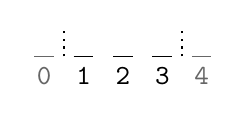
\begin{tikzpicture}
            \foreach \x in {0, 4} {
                \draw[opacity=0.6] (\x*0.5, 0) -- (\x*0.5+0.25, 0);
                \node[opacity=0.6] at (\x*0.5+0.125, -0.25) {\texttt{\x}};
            }
            \foreach \x in {1, 2, 3} {
                \draw (\x*0.5, 0) -- (\x*0.5+0.25, 0);
                \node at (\x*0.5+0.125, -0.25) {\texttt{\x}};
            }

            \draw[thick, dotted] (0.375, 0) -- (0.375, 0.35);
            \draw[thick, dotted] (1.875, 0) -- (1.875, 0.35);
        \end{tikzpicture}
        \caption{}
    \end{subfigure}
    \hfill
    \begin{subfigure}{0.3\textwidth}
        \centering
        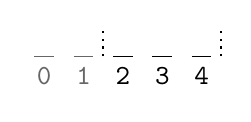
\begin{tikzpicture}
            \foreach \x in {0, 1} {
                \draw[opacity=0.6] (\x*0.5, 0) -- (\x*0.5+0.25, 0);
                \node[opacity=0.6] at (\x*0.5+0.125, -0.25) {\texttt{\x}};
            }
            \foreach \x in {2, 3, 4} {
                \draw (\x*0.5, 0) -- (\x*0.5+0.25, 0);
                \node at (\x*0.5+0.125, -0.25) {\texttt{\x}};
            }

            \draw[thick, dotted] (0.875, 0) -- (0.875, 0.35);
            \draw[thick, dotted] (2.375, 0) -- (2.375, 0.35);
        \end{tikzpicture}
        \caption{}
    \end{subfigure}
    \hfill
    \begin{subfigure}{0.3\textwidth}
        \centering
        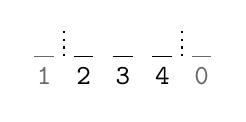
\begin{tikzpicture}
            \foreach \x[evaluate={int(mod(\x, 5))} as \y] in {5, 1} {
                \draw[opacity=0.6] (\x*0.5, 0) -- (\x*0.5+0.25, 0);
                \node[opacity=0.6] at (\x*0.5+0.125, -0.25) {\texttt{\y}};
            }

            \foreach \x in {2, 3, 4} {
                \draw (\x*0.5, 0) -- (\x*0.5+0.25, 0);
                \node at (\x*0.5+0.125, -0.25) {\texttt{\x}};
            }

            \draw[thick, dotted] (0.875, 0) -- (0.875, 0.35);
            \draw[thick, dotted] (2.375, 0) -- (2.375, 0.35);
        \end{tikzpicture}
        \caption{}
    \end{subfigure}
    \caption{The transition process for tape entries.}
    \label{fig:tape_movement}
\end{figure}

For the tape movement animation to look smooth, there are always 2 tape entries to either side of the tape. That way, if the tape gets moved to left or right, there will be a tape entry to show. This is illustrated in Figure \ref{fig:tape_movement} (a)- the tape entries 0 and 4 are out of frame and therefore invisible. 

When the tape moves, there will be 2 tape entries on one side. For instance, if the tape moves to the left in Figure \ref{fig:tape_movement} (a), we get Figure \ref{fig:tape_movement} (b). After the transition has completed, we move the most extreme tape entry to the other side. In the example, we move tape entry 0 to the right, leading to the tape state given in Figure \ref{fig:tape_movement} (c). At this point, we also change the tape value of entry 0 so that it matches tape value at index 5. Since these changes are invisible, they take place instantly after the animation is complete.
